\documentclass{article}

\usepackage{amsmath, graphicx}
\graphicspath{ {./images/} }

\title{HW 10.4 Solutions}
\author{Principles of Microeconomics}
\date{\today}

\begin{document}

\maketitle

\subsection*{Mankiw}

\begin{enumerate}
\setcounter{enumi}{8}

\item

\end{enumerate}

\subsection*{Non-Mankiw}

\begin{enumerate}

\item 

	\begin{enumerate}
	
	\item The value each firm places on a permit is equal to the cost the permit saves them by allowing them to pollute. That means Firm B values them the most and C the least. Firm B buys all of Firm C's permits for some price between \$10 and \$30 because Firm B is willing to pay more than the \$10 value that Firm C places on the permits. After buying 20 permits, Firm B can continue to produce its original 40 units of pollution, so it doesn't buy any more from Firm A. As a result, Firm A keeps its 20 permits. 

Since Firm C ends up with no permits, they spend $20 \cdot \$10 = \$200$ reducing their pollution. Since Firm A ends up with 20, they spend $10 \cdot \$20 = \$200$ reducing their pollution. Since Firm B ends up with 40 permits, they don't reduce their pollution. That means the total cost is \$400.

	\item Firm A would have spent $10 \cdot \$20 = \$200$ reducing their pollution. Firm B would have spent $20 \cdot \$30 = \$600$ reducing their pollution. Firm C would have spent \$0 reducing their pollution because they would have enough permits to cover their pollution. That means the total cost would be \$800.

	\end{enumerate}
	
\item

	\begin{enumerate}
	
	\item
		\begin{align*}
		50P_{mkt} &= 200 - 50P_{mkt} \\
		100P_{mkt} &= 200 \\
		P_{mkt} &= 2 \\
		Q_{mkt} &= 50(2) \\
		&= 100
		\end{align*}
		
	\item
		\begin{align*}
		50(P_{optimum}-2) &= 200 - 50P_{optimum} \\
		100P_{optimum} &= 300 \\
		P_{optimum} &= 3 \\
		Q_{optimum} &= 200 - 50(3) \\
		&= 50
		\end{align*}
		
		\begin{center}
		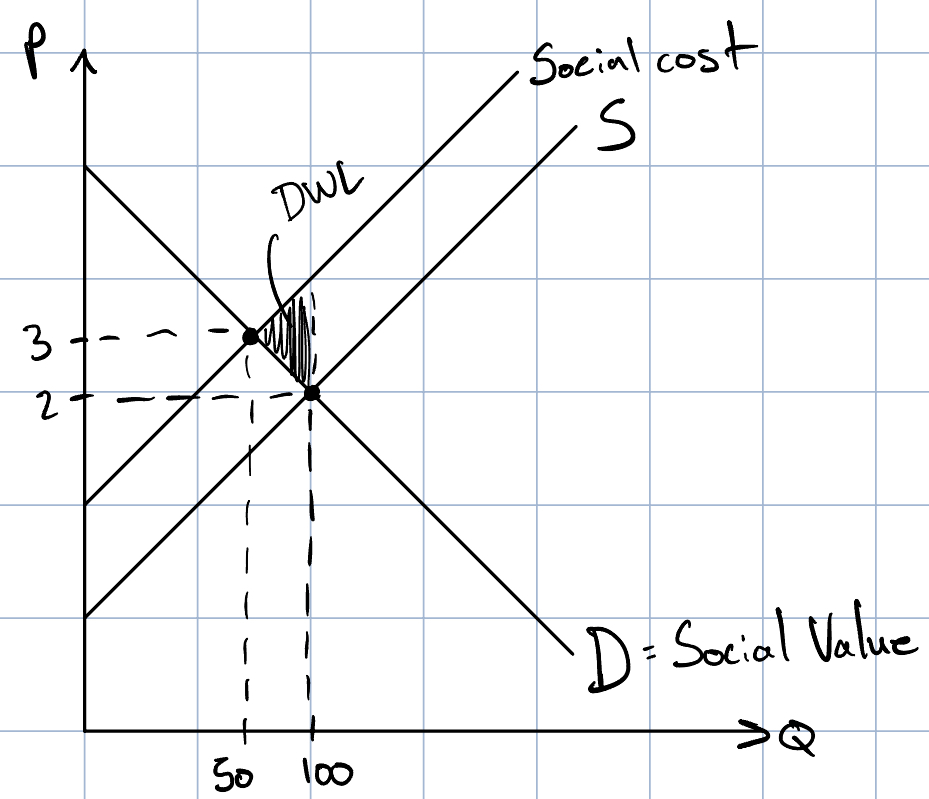
\includegraphics[width = 0.5\textwidth]{q1b}
		\end{center}
		
	\item Yes, there is dead weight loss because too many toys are made. Buyers and sellers have no incentive to consider the external costs the toys create for others, so they supply and demand too many of them. 
	
	\end{enumerate}

\end{enumerate}

\end{document}